\chapter{CoAP} \label{CoAP}

\section{Wat is CoAP?}

CoAP is een \textit{web transfer protocol} speciaal ontwikkeld voor netwerkcomponenten die beperkt zijn in zowel geheugen als energieverbruik, en voor \textit{machine-to-machine} (M2M)\nomenclature{M2M}{Machine-to-machine}-communicatie. Met M2M-communciatie bedoelen we communciatie tussen machines waar geen menselijke tussenkomst nodig is. Zoals de berichten die routers naar mekaar sturen om hun routingtabel te synchroniseren. Naast het minimaliseren van \textit{overhead} concentreert CoAP zich ook op het automatiseren van taken. Het mechanisme van resource \textit{discovery} (Zie paragraaf \ref{resourceDiscovery}) is hier een voorbeeld van. Met het verminderen van energieverbruik in het achterhoofd biedt CoAP naast synchrone ook asynchrone communicatie aan. Het biedt ook nieuwe soorten berichten aan zoals \textit{non-confirmable}, \textit{piggy-backed}, etc. Deze worden toegelicht in paragraaf \ref{betrouwbaarheid}\\


Het interactiemodel van CoAP is vergelijkbaar met het \textit{client}/servermodel van HTTP. Hoewel, bij een CoAP-implementatie voor M2M interacties kan een \textit{device} bij de ene berichtuitwisseling \textit{client} zijn, en bij de andere server. Een CoAP-\textit{request} is equivalent aan een HTTP-\textit{request} en wordt ook gestuurd van de \textit{client} naar de server om een actie aan te vragen op een resource die zich op die server bevindt. De actie wordt bepaald door een method code (GET, PUT, POST of DELETE) en de resource wordt aangeduid met een Uniform Resource Identifier (URI).\nomenclature{URI}{Uniform Resource Identifier} De server antwoordt met een response die onder andere een response code bevat.\\

Verschillend met HTTP, gebeurt de berichtenuitwisseling asynchroon over een datagram-ge\"{o}ri\"{e}nteerd transport. Dit houdt in dat berichten mogelijks verloren gaan of in een andere volgorde kunnen aankomen dan dat ze verzonden zijn. Toch voorziet CoAP enige vorm van betrouwbaarheid met een soort bericht dat kan worden bevestigd door een \textit{Acknowledgement} (zie paragraaf \ref{betrouwbaarheid}). Wanneer zo'n bericht niet wordt bevestigd, wordt het bericht meermaals opnieuw gestuurd volgens het \textit{exponential back-off}mechanisme (Zie paragraaf \ref{exponentialBackoff}).

CoAP definieert vier soorten berichten: \textit{Confirmable}, \textit{Non-confirmable}, \textit{Acknowledgement} en \textit{Reset}. Door gebruik te maken van method codes en response codes transporteren sommige van deze berichten \textit{requests} of responses. In paragraaf \ref{communicatieMogelijkheden} gaan we hier dieper op in.\\

\begin{wrapfigure}{r}{0.5\textwidth}
\vspace{-10pt}
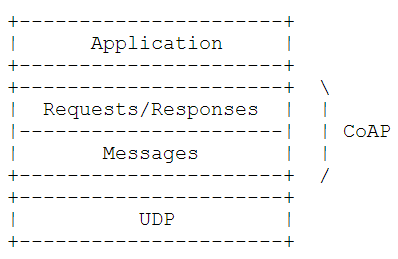
\includegraphics[width=0.5\textwidth]{fig/CoAPLaag}
\vspace{-30pt}
\caption{CoAP-lagen (CoAP 17 draft)}
\vspace{-5pt}
\label{fig:CoAPLaag}
\end{wrapfigure}
We kunnen CoAP ook in het \textit{Open Systems Interconnection} (OSI)-model \nomenclature{OSI}{Open Systems Interconnection} met 7 lagen plaatsen. Logisch gezien hebben we een CoAP-berichtenlaag die het UDP gedeelte en de asynchroniteit van de berichten afhandelt en een \textit{request}/responselaag die gebruik maakt van method en response codes (zie Figuur~\ref{fig:CoAPLaag}). Nochtans bestaat CoAP in werkelijkheid slechts uit \'{e}\'{e}n laag waarbij berichtenuitwisseling en het \textit{request}/responsemechanisme enkel en alleen door manipulatie van de \textit{header} verwezenlijkt wordt.

\subsection{Berichtformaat}

\begin{wrapfigure}{r}{0.7\textwidth}
\vspace{-20pt}
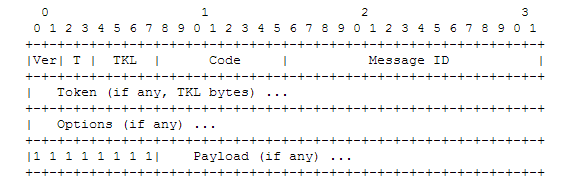
\includegraphics[width=0.7\textwidth]{fig/CoAPMessageFormat}
\vspace{-30pt}
\caption{Berichtformaat (CoAP 17 draft)}
\vspace{-10pt}
\label{fig:CoAPMessageFormat}
\end{wrapfigure}
Om een minimale \textit{overhead} te realiseren worden de berichten zeer compact gehouden. We geven een kort overzicht van de onderdelen van het berichtformaat (zie Figuur~\ref{fig:CoAPMessageFormat}) en bespreken dan de belangrijke delen apart in subparagrafen. De eerste vier bytes stellen de \textit{header} voor. Bemerk dus dat de \textit{header} gerealiseerd wordt met slechts 4 bytes. Het veld na de \textit{header} is optioneel en bevat een \textit{\textit{token}} waarvan de lengte aangegeven is in de \textit{header}. Vervolgens zitten er nul of meer opties in het bericht.
Het laatste onderdeel van een bericht is de \textit{payload}. Indien er een \textit{payload} aanwezig is in het bericht, wordt die altijd voorafgegaan door een vaste byte, de \textit{payload}marker (0xFF). Deze geeft het einde van de opties en het begin van de \textit{payload} aan. Indien er geen \textit{payload} is mag deze marker niet aanwezig zijn.

We merken hier op dat een \textit{token}, opties en een \textit{payload} optioneel zijn. Dit zorgt ervoor dat sommige berichten beperkt blijven tot de \textit{header} van 4 bytes, wat relatief weinig is.

\subsubsection{Header}

Deze vier bytes worden opgedeeld in drie delen:
\begin{itemize}
\item Versiegetal (Ver): een 2-bit \textit{unsigned integer} die de CoAP-versie aangeeft. 
\item Type-aanduiding (T): een 2-bit \textit{unsigned integer} die het berichttype aangeeft. De mogelijkheden zijn: \textit{confirmable} (CON) \nomenclature{CON}{Confirmable CoAP-message} (0), \textit{non-confirmable} (NON)) \nomenclature{NON}{Non-confirmable CoAP-message} (1), \textit{Acknowledgement} (ACK) \nomenclature{ACK}{Acknowledgement CoAP-message} (2) of \textit{Reset} (RST) \nomenclature{RST}{Reset CoAP-message} (3).
\item \textit{token}lengte (TKL)\nomenclature{TKL}{\textit{ToKen Length}}: een 4-bit \textit{unsigned integer} die de variabele \textit{token}lengte aangeeft.
\item Code: 8-bit \textit{unsigned integer} die aangeeft of het bericht een \textit{request} of een response overbrengt, of leeg is.
\item \textit{message-ID}: een 16-bit \textit{unsigned integer} die gebruikt wordt om duplicatie van berichten op te merken. Het wordt ook gebruikt om berichten van het type ACK/RST te linken aan berichten van het type CON/NON.
\end{itemize}

\subsubsection{Token}

Een \textit{token} wordt gebruikt om een response te linken aan een \textit{request}. De lengte wordt bepaald door de TKL en is nul tot acht bytes lang. Elk bericht heeft een \textit{token}, dit kan lengte nul hebben. Wanneer een \textit{token} nodig is, moet dat worden gegenereerd door de \textit{client}. Indien de server wil dat zijn response geaccepteerd wordt, moet hij dit \textit{token} zonder meer overnemen in zijn response.

\subsubsection{Opties}

%\begin{wrapfigure}{r}{0.6\textwidth}
%\vspace{-20pt}
%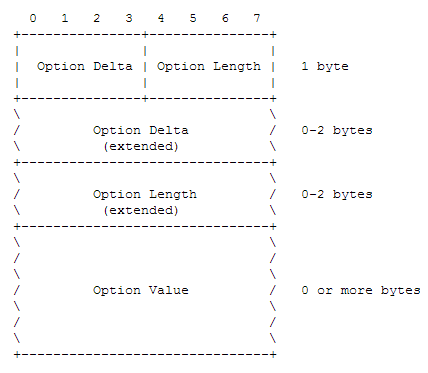
\includegraphics[width=0.6\textwidth]{fig/CoAPOpties}
%\vspace{-40pt}
%\caption{CoAP-optie (CoAP 17 draft)}
%\vspace{-10pt}
%\label{fig:CoAPOpties}
%\end{wrapfigure}
Opties worden opgesteld door middel van de Type-Length-Value (TLV)\nomenclature{TLV}{Type Length Value} notatie (zie Figuur~\ref{fig:CoAPOpties}). Er wordt een mechanisme toegepast om opties in een pakket te stoppen, dat ervoor zorgt dat het pakket compact blijft en dus bijdraagt tot een minimale \textit{overhead}.\\

Elke optie heeft een uniek nummer, maar wanneer meerdere opties in \'{e}\'{e}n pakket worden gestopt, worden de opties niet door dat nummer aangeduid, maar door de \textit{Option Delta}. De \textit{Option Delta} is het verschil tussen het nummer van een optie en dat van de vorige optie.
Concreet, stel dat men na een optie met nummer 6 een optie met nummer 11 wil plaatsen, dan wordt deze laatste aangeduid met \textit{Option Delta} gelijk aan 5 (11 - 6). Dit alles samen maakt dat een minimale (lege, maar daarom niet nutteloze) optie slechts 1 byte in beslag neemt. Dit heeft als gevolg dat opties na elkaar moeten worden geplaatst met oplopende optienummers.\\

Er zijn gevallen dat dit systeem tekort schiet. Daarom zijn er speciale waarden ingevoerd die het gebruik van een \textit{extended Option Delta} aangeven. Indien de \textit{Option Delta} groter is dan 12, maar kleiner is dan 269, wordt als \textit{Option Delta} waarde 13 gebruikt. Er wordt dan een extra byte voor de Option Value gezet dat opgevuld wordt met de echte \textit{Option Delta} - 13. Indien de Option delta meer is dan 268, wordt als \textit{Option Delta} de waarde 14 gebruikt. Deze waarde geeft aan dat er twee extra bytes gebruikt worden. Deze bytes worden opgevuld met de echte \textit{Option Delta} - 269. De waarde 15 mag niet als \textit{Option Delta} gebruikt worden want deze geeft het begin van de \textit{payload} aan. Voor Option Length zijn de regels analoog.


\begin{figure}[h]
\centering
%\vspace{10pt}
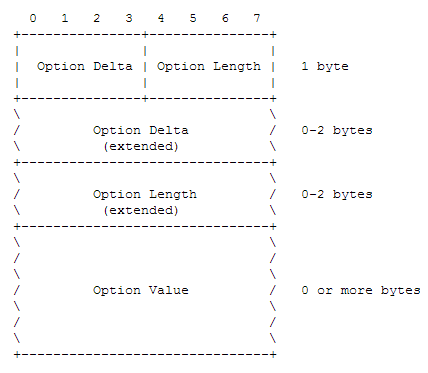
\includegraphics[width=0.6\textwidth]{fig/CoAPOpties}
\vspace{-10pt}
\caption{CoAP-optie (CoAP draft 16)}
\label{fig:CoAPOpties}
\end{figure}

\newpage

\subsubsection{Verschil met HTTP}

Als we dit kort vergelijken met het berichtformaat van HTTP (zie Figuur~\ref{fig:HTTPMessageFormat}) zien we dat er aanzienlijke verschillen zijn. Bij HTTP zijn \textit{request} en response niet helemaal gelijk. We kijken eerst naar de HTTP-\textit{request} die opgedeeld is in drie delen:
\begin{itemize}
\item Een \textit{request}lijn die op zijn beurt opgedeeld is in drie delen gescheiden door een spatie:
\begin{itemize}
\item de methodenaam (GET, POST, HEAD, PUT of DELETE voor HTTP 1.1)
\item de URL van de gevraagde resource
\item het versienummer
\end{itemize}
\item Een aantal \textit{header}lijnen die bijkomende opties voorstellen.
\item De entity body wordt gebruikt door de POST-methode om gegevens door te sturen en wordt gescheiden van de \textit{header}lijnen door een lege lijn. 
\end{itemize}
Bijkomend wordt elke lijn (ook de lege) afgesloten met een \textit{carriage return} (CR)\nomenclature{CR}{Carriage Return} en een \textit{line feed} (LF\nomenclature{LF}{Line Feed}).

De HTTP-response is analoog aan de \textit{request} met als verschillen dat de eerste lijn opgebouwd is uit het versienummer, de statuscode die aangeeft wat het resultaat van de \textit{request} inhoudt en een korte beschrijving van de statuscode.\\
Het is dus duidelijk dat een HTTP-bericht aanzienlijk groter zal zijn dan een CoAP-bericht.

\begin{figure}[h]
\vspace{10pt}
\centering
\subcaptionbox{Request}
{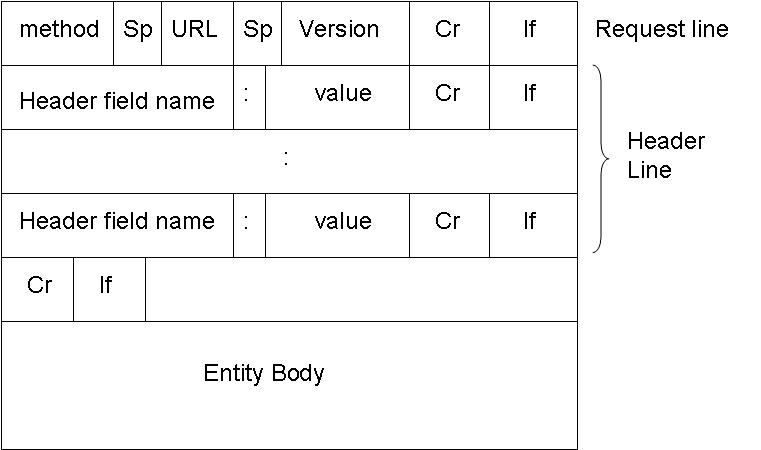
\includegraphics[width=0.45\textwidth]{fig/HTTPRequestMessageFormat}}
\subcaptionbox{Response}
{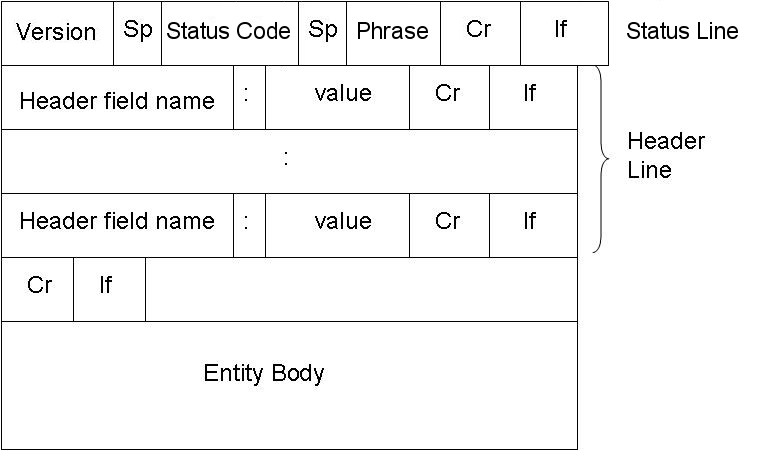
\includegraphics[width=0.45\textwidth]{fig/HTTPResponseMessageFormat}}
\caption{HTTP-berichtformaat}
\label{fig:HTTPMessageFormat}
\end{figure}

\newpage

\section{Communicatiemogelijkheden} \label{communicatieMogelijkheden}

In deze paragraaf bespreken we de communicatiemogelijkheden van CoAP. We bekijken de variabele betrouwbaarheid van CoAP-berichten en gaan na hoe het \textit{request}/responsemodel bij CoAP werkt aan de hand van voorbeelden. Als laatste lichten we het principe van \textit{blockwise transfer} toe.

\subsection{Betrouwbaarheid} \label{betrouwbaarheid}

HTTP realiseert een betrouwbare en robuuste vorm van communicatie. Het is gebaseerd op het \textit{Transmission Control Protocol} (TCP). Dit protocol zet een verbinding op aan de hand van \textit{stream sockets}. Het zorgt ervoor dat pakketten gegarandeerd aankomen bij de bestemming en dit in volgorde van verzending. Maar deze betrouwbaarheid komt met een prijs, namelijk extra netwerkbelasting voor het opzetten en beheren van die verbinding. In tegenstelling tot HTTP dat gebouwd is op TCP, is CoAP gebaseerd op berichtenuitwisseling over UDP. Wanneer men met dit protocol werkt, is er echter geen garantie dat pakketten aankomen en wanneer dat wel het geval is, kan de volgorde van aankomst gewijzigd zijn ten opzichte van verzending. Daarom moet men bij CoAP zelf de betrouwbaarheid verzorgen indien nodig.

\subsubsection{Confirmable berichten}

Wanneer we de betrouwbaarheid van de berichtenuitwisseling willen opdrijven, merken we de berichten als CON. Een CON-bericht moet door de server worden beantwoord met een ACK-bericht (zie Figuur~\ref{fig:berichtuitwisseling}), dit ACK-bericht moet hetzelfde \textit{message-ID} bevatten als het CON-bericht waarop geantwoord wordt. Wanneer CON-berichten niet worden beantwoord met een ACK-bericht v\'{o}\'{o}r een bepaalde time-out, wordt het bericht opnieuw verzonden. Bij het opnieuw verzenden wordt een \textit{exponential back-off}mechanisme toegepast. Eerst wordt een time-out bepaald tussen een ACK\_TIMEOUT en ACK\_TIMEOUT x ACK\_RANDOM\_FACTOR, wanneer die time-out verstrijkt wordt het CON-bericht opnieuw verzonden en de time-out verdubbeld. Wanneer de server niet in staat is het CON-bericht te verwerken, wat betekent dat die zelfs geen geldige \textit{error}response kan geven, antwoordt die met een RST-bericht in plaats van met een ACK-bericht.

\subsubsection{Non-confirmable berichten}

Soms heeft een bericht geen betrouwbaar transport nodig. Een voorbeeld hiervan is een stroom van sensordata waarbij elke meting verstuurd wordt met een NON-bericht. Dit soort berichten wordt niet bevestigd met een ACK bericht, maar de berichten hebben wel nog steeds een \textit{message-ID} om duplicatie van berichten te detecteren (zie Figuur~\ref{fig:berichtuitwisseling}). Wanneer een ontvanger niet in staat is het bericht te verwerken, opnieuw bedoelen we daarmee dat het geen geldige \textit{error}response kan geven, zendt die een RST-bericht naar de zender.

\begin{figure}[h]
\vspace{10pt}
\centering
\subcaptionbox{Confirmable}
{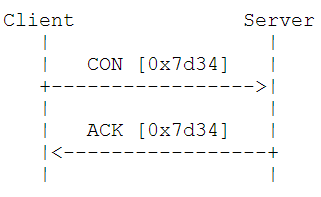
\includegraphics[width=0.3\textwidth]{fig/CoAPConfirmable}}
\hspace{30pt}
\subcaptionbox{Non-confirmable}
{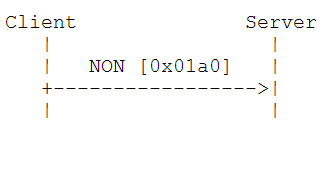
\includegraphics[width=0.3\textwidth]{fig/CoAPNonConfirmable}}
\caption{Berichtuitwisseling (CoAP 17 draft)}
\label{fig:berichtuitwisseling}
\end{figure}

\subsection{Request/responsemodel}

\subsubsection{Piggy-backed response}

Wanneer een \textit{request} met een CON-bericht verstuurd wordt, is het mogelijk dat het antwoord meteen beschikbaar is bij de server. Indien dit het geval is, wordt het antwoord op de \textit{request} meteen meegestuurd met het ACK-bericht. Dit wordt een \textit{piggy-backed} response genoemd. In Figuur~\ref{fig:CoAPPiggyBacked} worden twee voorbeelden van GET-\textit{requests} met \textit{piggy-backed} responses getoond. De ene is succesvol, de andere geeft een \textit{error}response terug.
\begin{figure}[h]
\vspace{10pt}
\centering
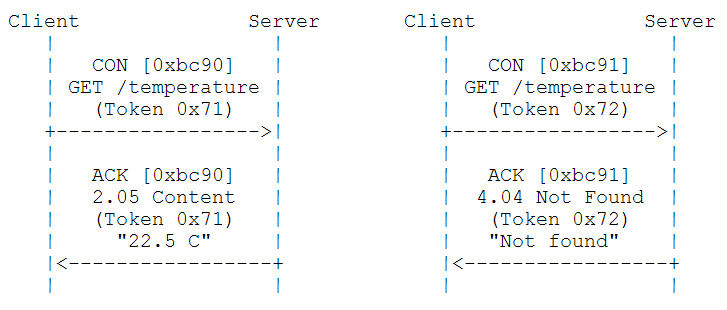
\includegraphics[width=0.7\textwidth]{fig/CoAPPiggyBacked}
%\vspace{-10pt}
\caption{Twee GET-requests met piggy-backed responses (CoAP 17 draft)}
\label{fig:CoAPPiggyBacked}
\vspace{-20pt}
\end{figure}

\newpage
\subsubsection{Separate response} \label{separate}

\begin{wrapfigure}{r}{0.3\textwidth}
\vspace{-40pt}
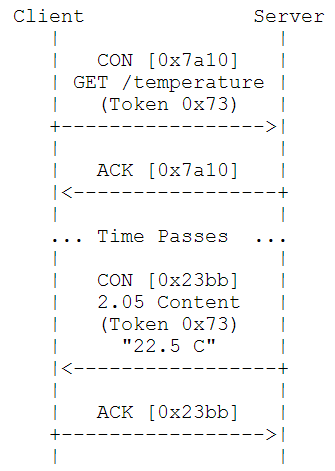
\includegraphics[width=0.3\textwidth]{fig/CoAPSeperateResponse}
\vspace{-30pt}
\caption{GET-request met separate response (CoAP 17 draft)}
\label{fig:SeparateResponse}
\vspace{-100pt}
\end{wrapfigure}
Wanneer de server niet onmiddellijk kan antwoorden op de \textit{request} van de \textit{client}, antwoordt die met een leeg ACK-bericht zodat de \textit{client} niet zou beginnen heruitzenden als gevolg van het \textit{exponential back-off}mechanisme. Wanneer de response klaar is, stuurt de server dit antwoord in een nieuw CON-bericht dat op zijn beurt beantwoord moet worden door de \textit{client}. Dit soort van berichtenuitwisseling heet \textit{separate} response (zie Figuur~\ref{fig:SeparateResponse}).
\\
\\
\\

\subsection{Blokken} \label{blocks}
CoAP werkt goed als de berichten geen of kleine \textit{payloads} bezitten. Dit mag je veronderstellen als je werkt met temperatuursensors of lichtschakelaars. Maar soms is het nodig dat applicaties berichten sturen met grotere \textit{payloads}, zoals bij resource \textit{discovery} dat we in \ref{resourceDiscovery} bespreken of bij resources die nu eenmaal veel gegevens als antwoord op een \textit{request} hebben.\\

Bij HTTP doet TCP al het werk om de pakketten te fragmenteren en ervoor te zorgen dat de deelpakketten in de juiste volgorde verwerkt worden. Dit is niet mogelijk bij CoAP aangezien UDP als transportprotocol gebruikt wordt. Bij UDP zijn er ook verschillende niveau's van fragmentatie mogelijk. Gebruik van deze niveau's moet vermeden worden om de fragmentatie af te handelen op applicatieniveau. Op deze manier worden meerdere blokken informatie van een enkele resource uitgewisseld via meerdere \textit{request}/responseparen. Belangrijk op te merken hierbij is dat elk \textit{request}/responsepaar afzonderlijk af te handelen is door \textit{client} en server. Dit heeft als gevolg dat er geen connectie opgezet moet worden en dat de server geen geheugen moet vrijmaken om bij te houden welke blokken hij al verstuurd heeft. Welke de niveau's zijn en waarom er voor de Block Options gekozen is wordt uitvoerig besproken in de draft '\textit{Blockwise transfers in CoAP}' \cite{blockwiseTransfer}.

\subsubsection{Block Options}
Om grote \textit{payloads} op een goede manier te ondersteunen worden twee Block Options ingevoerd. Optie 23 heeft als naam Block2 en geeft informatie over de \textit{payload} van de \textit{request}. Optie 27 heeft als naam Block1 en geeft informatie over de \textit{payload} van de response. Beide opties  geven een \textit{blockwise transfer} aan en kunnen zowel in een \textit{request} als in een response voorkomen. Ze ondersteunen blokgroottes die een macht van twee zijn, beginnend bij 16 t.e.m. 1024 bytes.

\subsubsection{Structuur}
Bij beide opties hebben de optiewaarden dezelfde structuur. De lengte van de waarde is variabel en kan 1, 2 of 3 bytes lang zijn zoals te zien is in figuur~\ref{fig:blockOption}.
\begin{figure}[h]
\centering
\includegraphics[width=0.6\textwidth]{fig/blockOption}
\caption{Blokoptiewaarde - bytes en bits worden aangegeven bovenaan de figuur}
\label{fig:blockOption}
\end{figure}

\noindent
Wat we nog uit figuur~\ref{fig:blockOption} halen is dat het telkens drie elementen bevat:
\begin{enumerate}
\item NUM (\textit{Block Number}): Het relatief nummer van het blok binnen een sequentie van blokken.
\item M (\textit{More Flag}): Is dit het laatste blok in een reeks?
\item SZX (\textit{Size Exponent}): Geeft de grootte van het blok.
\end{enumerate}

\noindent
De blokgrootte is ge\"{e}ncodeerd gebruik makend van een drie-bit \textit{unsigned integer}. 0 komt overeen met $ 2^{4} $ en 6 komt overeen met  $ 2^{10} $. Concreet wordt de grootte van het blok gegeven door  $ 2^{ SZX + 4} $. 7 mag niet gebruikt worden als waarde omdat deze gereserveerd is.

\section{Extra Features}

\subsection{Observe} \label{observe}

Wanneer een resource \textit{observable} is of anders gezegd, de \textit{ovserve}functionaliteit ondersteunt, kan die resource op eigen initiatief data sturen naar eventueel ge\"{i}nteresseerde \textit{clients}. Een \textit{client} kan zijn interesse uiten door een CON-bericht met een lege \textit{observe}-optie (optie 6) naar de server te sturen. Wanneer de \textit{client} dan een ACK-bericht terug krijgt met een \textit{observe}-optie, weet die dat de server de \textit{client} heeft toegevoegd aan de lijst van \textit{observers}. Een \textit{client} kan aangeven aan de server dat die niet meer ge\"{i}nteresseerd is door een RST-bericht te sturen naar de server. De server verwijdert de \textit{client} dan uit de lijst van ge\"{i}nteresseerden.

\subsection{Resource discovery} \label{resourceDiscovery}
Resource \textit{discovery} zorgt ervoor dat lokale \textit{client} en servers elkaar kunnen vinden en met elkaar kunnen interageren zonder menselijk tussenkomst.

\subsubsection{Principe}
\noindent
Resources kunnen maar aangesloten zijn op \'{e}\'{e}n \textit{device}. Dit \textit{device} maakt een extra resource aan met als naam '\textit{well-known/core}'. Deze extra resource bevat een opsomming van alle resources verbonden met dit \textit{device} en een aantal gegevens over deze resources onder de vorm van attributen. Sommige \textit{well-known/core}'s bevatten ook verwijzingen naar resources op andere \textit{device}s. Gebruikers kunnen een GET-\textit{request} sturen om de \textit{well-known/core} op te halen en hebben dan deze informatie tot hun beschikking. De \textit{well-known/core} bevat echter veel informatie die niet in een enkel \textit{request}/responsepaar uitgewisseld kan worden. Daarom wordt er gebruik gemaakt van blokken, welke uitgelegd worden in \ref{blocks}. De manier waarop deze informatie doorgegeven wordt, is door gebruik te maken van het \textit{CoRE Link Format} \cite{coapDiscovery}.

\subsubsection{CoRE Link Format}
Er worden geen resources opgeslaan in de \textit{well-known/core} maar links naar resources. Als formaat van de links moet het \textit{CoRE Link Format} gebruikt worden. Een resource wordt binnen het device uniek ge\"{i}dentificeerd door een \textit{target}-URI. De \textit{target}-URI in combinatie met de URI van het device vormt de URI van de resource waarmee hij globaal uniek ge\"{i}dentificeerd wordt. Deze \textit{target}-URI staat tussen een kleiner-dan (\textless) en een groter-dan (\textgreater) teken. Na de URI worden alle attributen opgesomd gescheiden door een puntkomma (;). De attributen zelf hebben de vorm van een naam-waardepaar. Sommige attributen kunnen meerdere waarden hebben, deze waarden worden dan gescheiden door een spatie. Tot slot worden verschillende links gescheiden met een komma (,).\\

\noindent
Als voorbeeld geven we het antwoord op een GET-\textit{request} van een \textit{well-known/core}:
\begin{verbatim}
</temp>;rt="temperature-c";if="sensor";ct="0 40",
</light>;rt="light-lux";if="sensor"
\end{verbatim}
We zien dat het \textit{device} met deze \textit{core} twee resources aanbiedt. De eerste resource wordt ge\"{i}dentificeerd met de \textit{target}-URI temp, de andere met light. De eerste resource heeft drie attributen en ondersteund twee \textit{content formats}. De tweede resource heeft twee attributen. Er zijn echter meer attributen mogelijk. We sommen enkele algemene attributen op:
\begin{itemize}
\item obs (\textit{Observable}): Geef aan of de resource \textit{observable} is. Indien de optie ontbreekt wordt aangenomen dat de resource niet \textit{observable} is.
\item rt (\textit{Resource Type}): Geeft het type van de resource. De waarden zijn afhankelijk van de gebruikte applicatie. Ze hebben als nut dat binnen een applicatie, resources van hetzelfde type herkent kunnen worden. Dan is het mogelijk via query filtering, alle resources van een type opgehaald worden. Meerdere waarden zijn mogelijk.
\item ct (\textit{Content Type}): Bevat een opsomming van de \textit{content formats} die ondersteund worden door deze resource. Meerdere waarden zijn mogelijk.
\item if (\textit{Interface Description}): Bevat een beschrijving van welke methoden deze resource ondersteunt. Meerdere waarden zijn mogelijk.
\item sz (\textit{Maximum Size Estimate}): Bevat een schatting van de maximale grootte van een response. Voor grote resources zou dit ge\"{i}mplementeerd moeten worden maar het is geen verplichting.
\item title: Bevat een omschrijving van de resource.
\item anchor: Wordt gebruikt om de link te laten verwijzen naar een willekeurige resource. Dit kan een resource binnen de eigen \textit{core} zijn of erbuiten. Het rel-attribuut wordt vaak samen met deze optie gebruikt om de relatie aan te duiden tussen de link en de resource. Implementaties die het vermogen niet hebben deze optie te verwerken moeten de hele link te negeren.
\item rel: Geeft de relatie tussen de link en de resource.
\end{itemize}
Al deze attributen mogen maar een keer voorkomen. De lijst met alle attributen vind je in de \textit{CoRE Link Format draft} \cite{coapDiscovery}. Maar niet alle beschrijvingen van deze attributen staan in de \textit{CoRE Link Format draft}. De ontbrekende beschrijvingen vind je in de \textit{Web Linking draft} \cite{webLinking}.

\subsubsection{Core ophalen}
Om een \textit{well-known/core} op te halen, moet je twee maal de Uri-Pathoptie (optie 11) toevoegen aan een GET-\textit{request} die gericht is naar het IP-adres van het \textit{device} waar de \textit{core} zich op bevindt. De eerste keer met als waarde 'well-known' en de tweede keer gebruik je 'core' als waarde.\\

\noindent
We bespreken de eerste berichtenparen bij een resource \textit{discovery} door de hexadecimale waarde te bekijken. Verschillende onderdelen binnen het bericht scheiden we met een streep.\\

\noindent
De \textit{client} stuurt een eerste \textit{discovery} \textit{request}:\\
40 01 78 a5 \textbar~bb 2e 77 65 6c 6c 2d 6b 6e 6f 77 6e \textbar~04 63 6f 72 65\\
Het eerste deel bevat dezelfde elementen als elke GET-\textit{request}. Het tweede deel bevat de eerste optie met als eerste twee bytes 'bb'. Dit komt overeen met optie 11 met lengte 11. De 11 volgende byteparen zijn de hexadecimale waarden van de karakters 'well-known'. Het laatste deel bevat ook een optie. Deze keer zijn de twee eerste bytes '04'. De \textit{Option Delta} is 0, dus hebben we opnieuw optie 11. De lengte is deze keer 4. De volgende byteparen komen overeen met 'core'.\\

\noindent
Het antwoord van de server:\\
60 45 78 a5 \textbar~c1 28 \textbar~b1 0c \textbar~52 06 92 \textbar~ff ...\\
Het eerste deel is analoog aan andere responseberichten. We merken wel op dat de \textit{message-ID} dezelfde is als de \textit{message-ID} in de \textit{request} van de \textit{client}. De eerste twee bytes van het tweede deel zijn 'c1'. Wat optie 12 (\textit{Content-Format}) met lengte 1 impliceert. De waarde van deze optie is 28. Omgezet naar decimaal is dit 40, wat application/link-format aangeeft. Het volgende deel begint met 'b1'. Dit komt overeen met optie 23 (Block2) met lengte 1. De hexadecimale waarde is '0c' wat overeenkomt met 12 of binair 00001100. Als we dit herschikken zien we de elementen die in figuur~\ref{fig:blockOption} te zien zijn: 0000 1 110. We zien dat dit het eerste blok is van een reeks van blokken met grootte 6 bytes. We zien ook dat er nog blokken aangevraagd moeten worden. Het voorlaatste deel begint met '52' wat optie 28 aanduidt met lengte 2. Optie 28 (\textit{Block Size}) mag genegeerd worden en wordt besproken in \ref{unsupportedBlockOptions}. Het laatste deel begint met de \textit{payload}marker waarop de \textit{payload} volgt.\\

\noindent
De \textit{client} stuurt een nieuwe \textit{request} om het volgende pakket op te vragen:\\
40 01 78 a6 \textbar~bb 2e 77 65 6c 6c 2d 6b 6e 6f 77 6e \textbar~04 63 6f 72 65 \textbar~c1 16\\
De eerste drie delen zijn analoog aan de eerste \textit{request}. Het laatste deel dat erbij is gekomen geeft het volgende blok aan dat verstuurd moet worden door de server. De eerste twee bytes zijn 'c1'. \textit{Option Delta} is 12 dus de optie is 11 + 12 = 23 (Block2). De lengte is 1 bytepaar. 16 binair is 0001 0 110. Het tweede blok in de reeks van blokken met lengte 6 bytes wordt opgevraagd.\\

\noindent
De server zal met het aangevraagde blok antwoorden. Dit proces blijft zich herhalen tot de server een response stuurt waar de M-bit op 0 staat.

\subsubsection{Query Filtering}
Het is mogelijk een specifieke resource \textit{discovery} uit te voeren indien er enkel informatie over een resource moet gekend zijn of enkel de resources waarbij een bepaald attribuut een specifieke waarde heeft. Dit heeft als voordeel dat het netwerk niet overbodig belast moet worden als dat niet nodig is. De \textit{query}filter wordt voorgesteld door een naam-waardepaar. Deze wordt toegevoegd door de \textit{Uri-Query}optie (optie 15) te gebruiken.

